\section{\scshape Sensors and environments modeling}

\begin{frame}{Depth sensors modeling}
	\begin{itemize}
		\item Modeling in the Gazebo simulator of 3D sensors with different technical characteristics:
		\begin{itemize}
			\item Resolution
			\item Field of view
			\item Minimum and maximum measurement range
			\item Sensor acquisition rate
		\end{itemize}
		\item Creation of simulation models for 3D sensors widely used from several manufacturers:
		\begin{itemize}
			\item Ensenso
			\item Kinect
			\item Realsense
			\item Orbbec
			\item ZED
		\end{itemize}
	\end{itemize}
\end{frame}


\begin{frame}{Environments modeling}
	\begin{itemize}
		\item Modeling of 4 different test environments:
		\begin{itemize}
			\item 1 for active perception with hand occlusions.
			\item 1 for bin picking with minimal occlusions.
			\item 1 for bin picking with large occlusions.
			\item 1 for multiple object bin picking with large occlusions.
		\end{itemize}
		\item Target object:
		\begin{itemize}
			\item Starter motor
		\end{itemize}
		\item Support and occluding objects:
		\begin{itemize}
			\item Large stacking box
			\item Trolley with shelves
			\item Differential gearbox
			\item Alternator
		\end{itemize}
		\item The target object model uses a special surface material that ignores light effects (such as shading) and has a unique color (green) that will be used for sensor data segmentation.
	\end{itemize}
\end{frame}


\begin{frame}{Environment for active perception}
	\begin{figure}
		\centering
		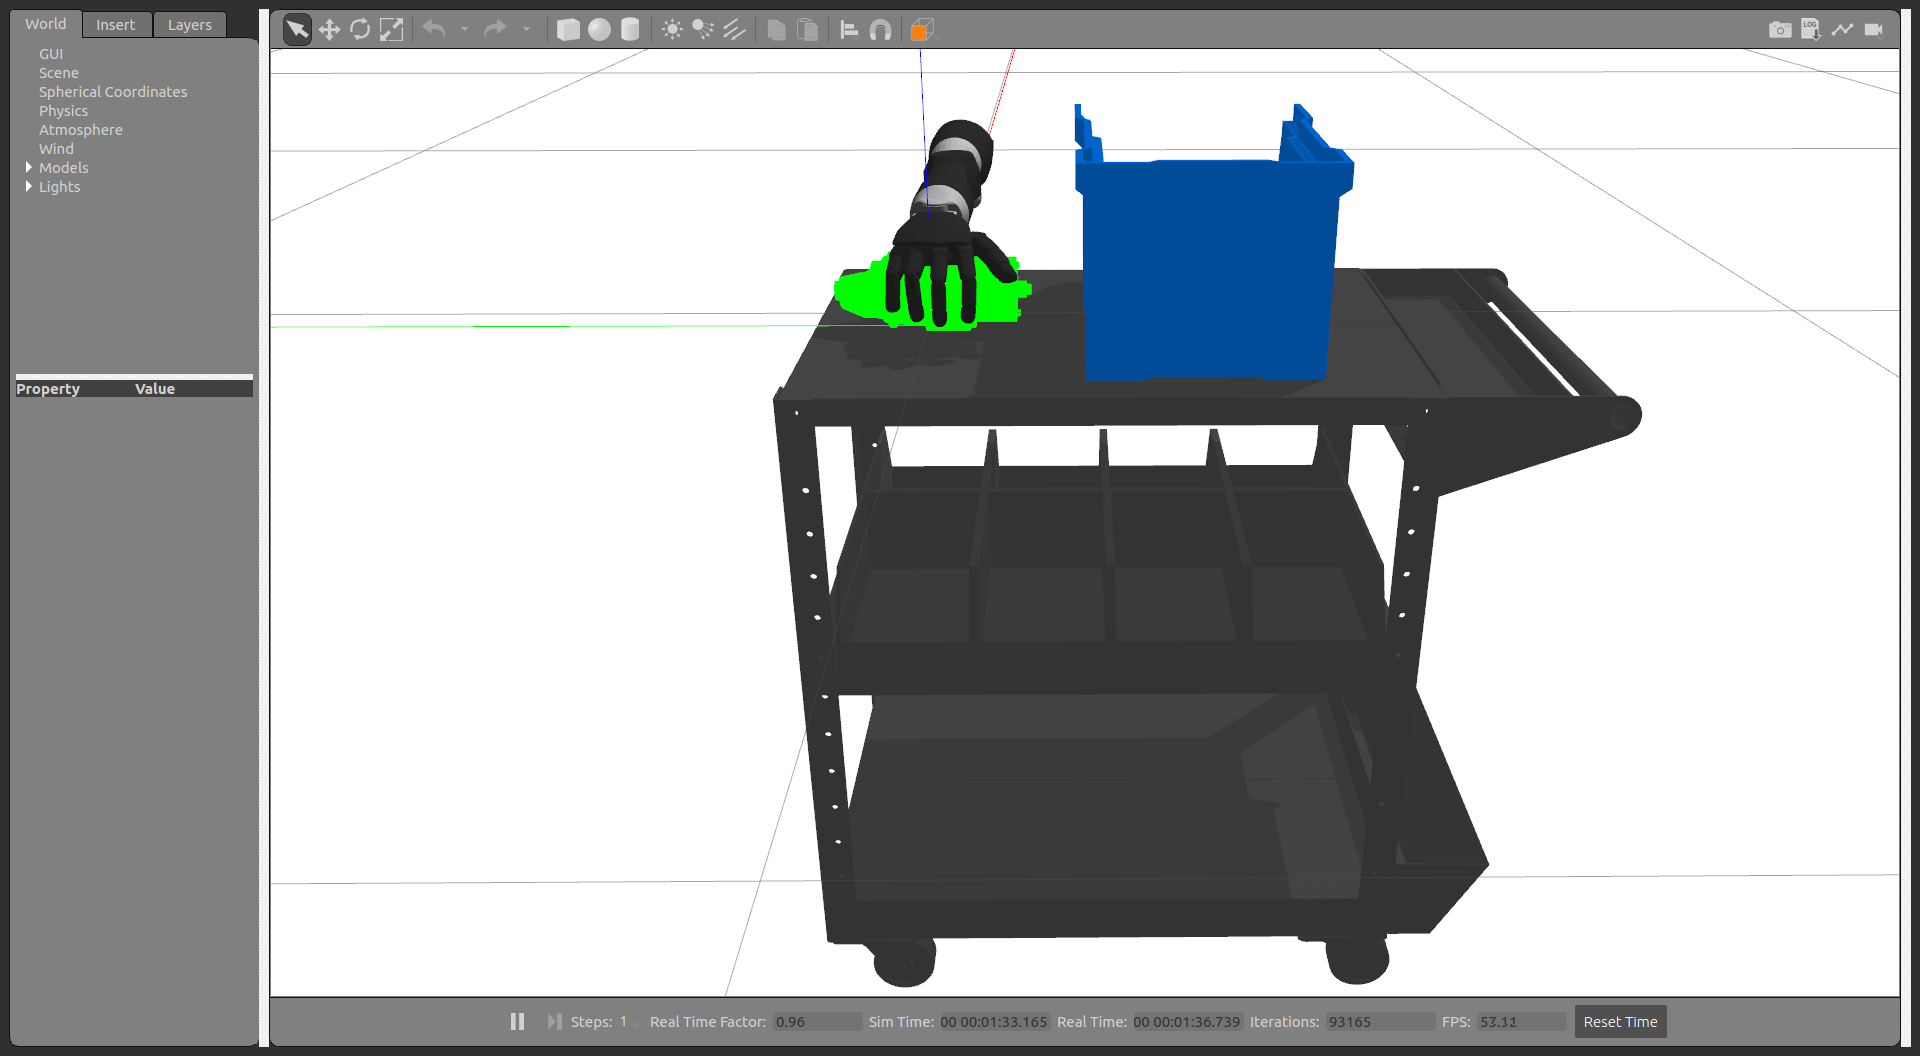
\includegraphics[height=.42\textheight]{environments/active-perception/gazebo-back}
		\includegraphics[height=.42\textheight]{environments/active-perception/gazebo-top}\\
		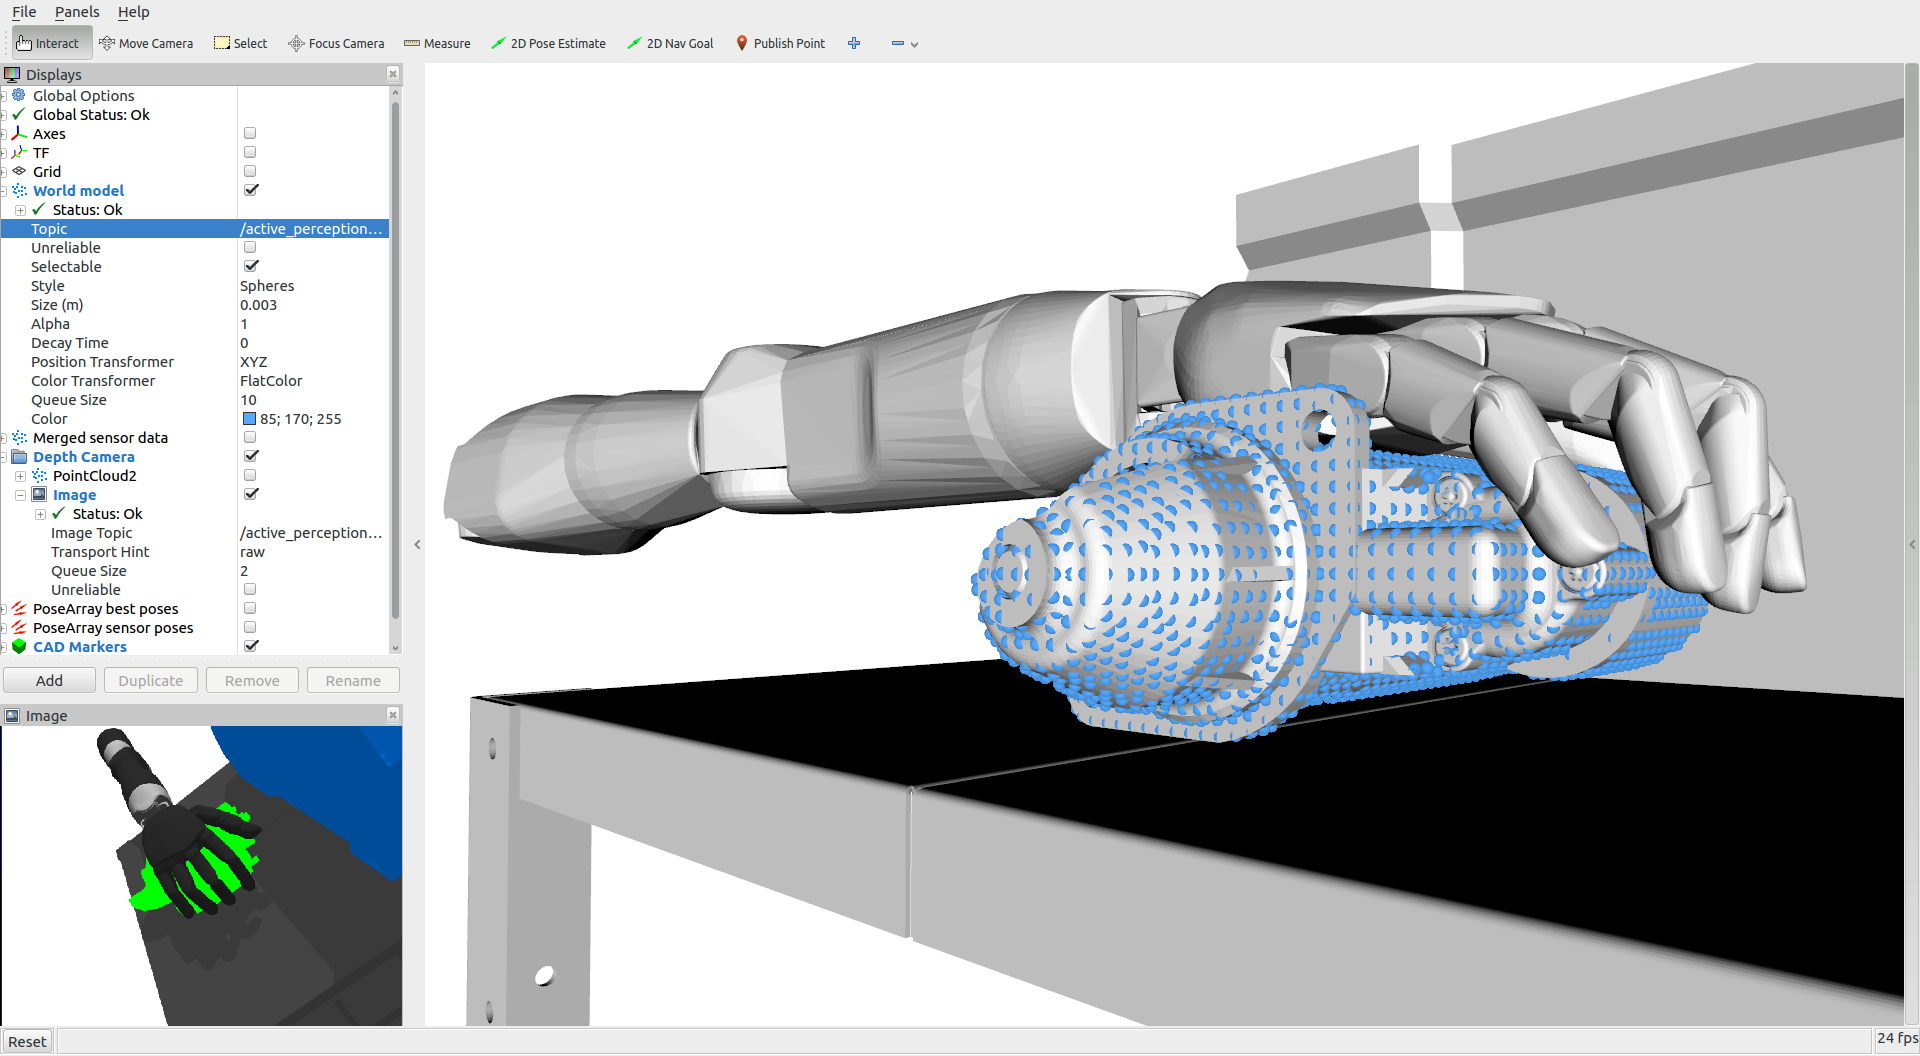
\includegraphics[height=.42\textheight]{environments/active-perception/rviz-back-left}
		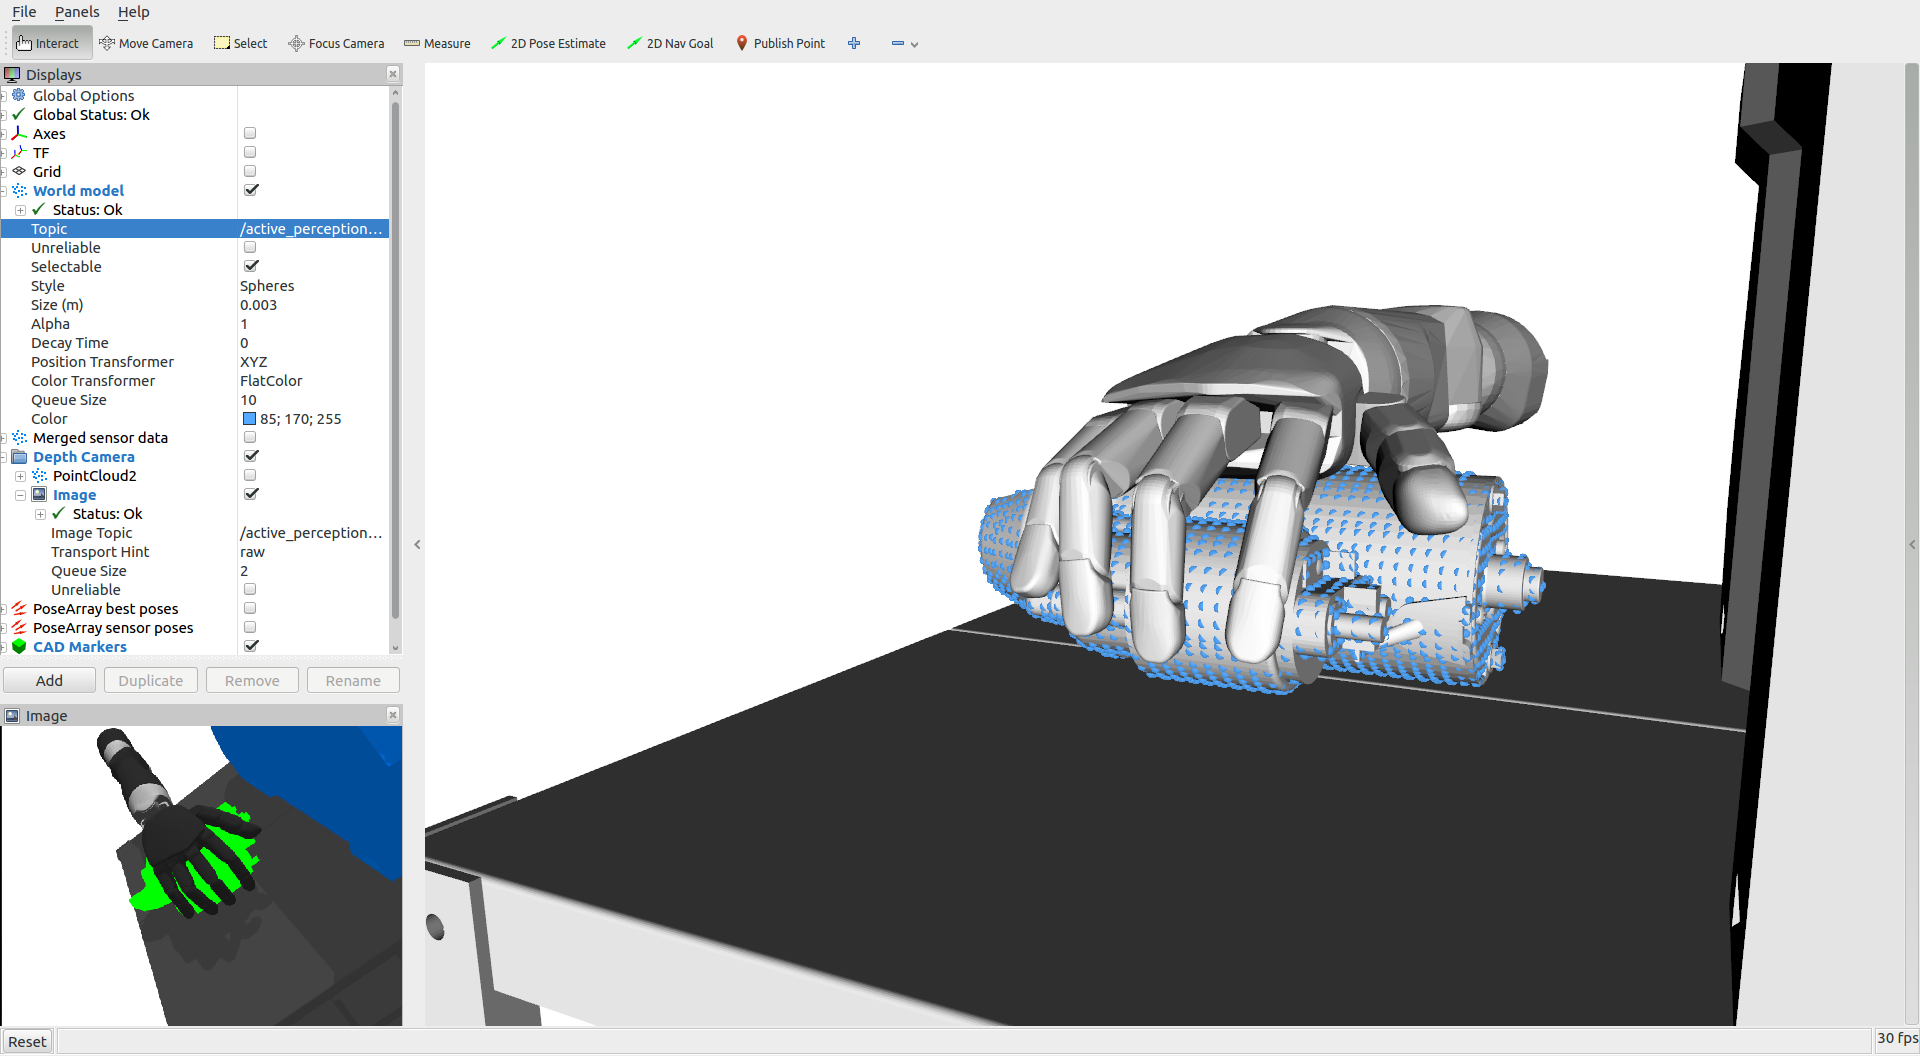
\includegraphics[height=.42\textheight]{environments/active-perception/rviz-back-right}
		\caption{Environment with a hand occluding a starter motor.}
	\end{figure}
\end{frame}


\begin{frame}{Environment for bin picking}
	\begin{figure}
		\centering
		\includegraphics[height=.42\textheight]{environments/bin-picking/gazebo-front}
		\includegraphics[height=.42\textheight]{environments/bin-picking/gazebo-top}\\
		\includegraphics[height=.42\textheight]{environments/bin-picking/rviz-front}
		\includegraphics[height=.42\textheight]{environments/bin-picking/rviz-top}
		\caption{Environment with a gearbox and an alternator occluding a starter motor.}
	\end{figure}
\end{frame}


\begin{frame}{Environment for bin picking with occlusions}
	\begin{figure}
		\centering
		\includegraphics[height=.42\textheight]{environments/bin-picking-with-occlusions/gazebo-front}
		\includegraphics[height=.42\textheight]{environments/bin-picking-with-occlusions/gazebo-top}\\
		\includegraphics[height=.42\textheight]{environments/bin-picking-with-occlusions/rviz-front}
		\includegraphics[height=.42\textheight]{environments/bin-picking-with-occlusions/rviz-top}
		\caption{Environment with gearboxes and an alternator occluding a starter motor.}
	\end{figure}
\end{frame}


\begin{frame}{Environment for multiple bin picking with occlusions}
	\begin{figure}
		\centering
		\includegraphics[height=.42\textheight]{environments/multiple-bin-picking-with-occlusions/gazebo-front}
		\includegraphics[height=.42\textheight]{environments/multiple-bin-picking-with-occlusions/gazebo-top}\\
		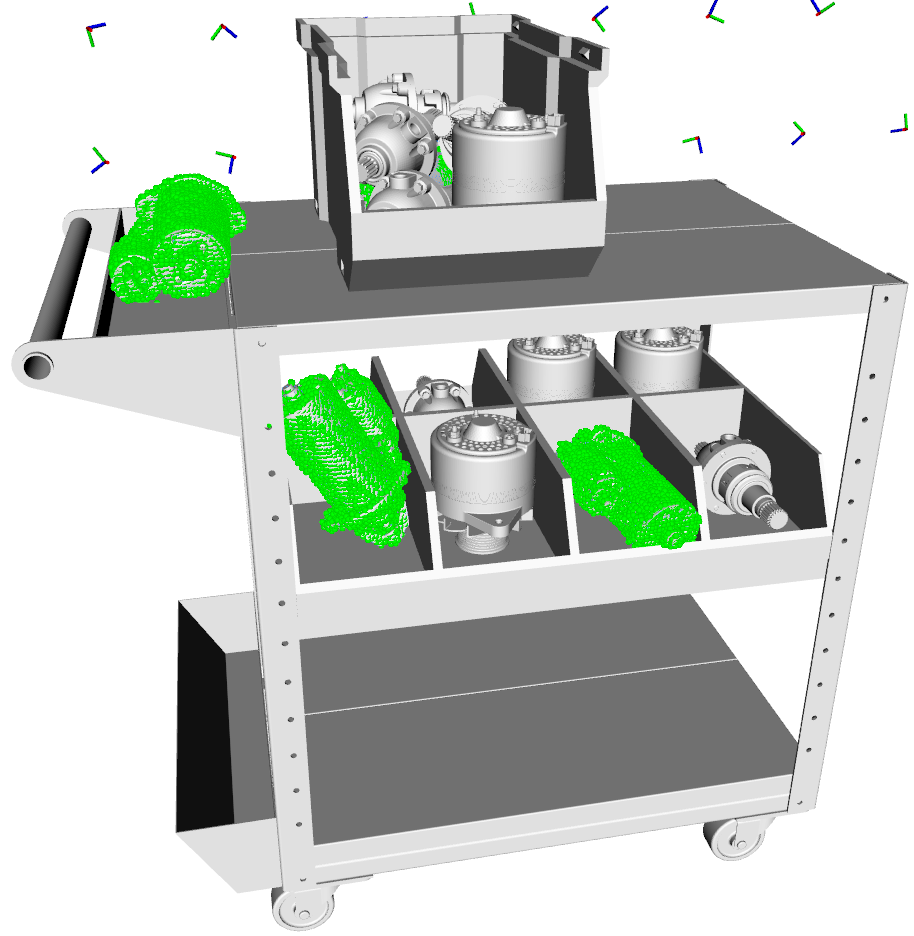
\includegraphics[height=.42\textheight]{environments/multiple-bin-picking-with-occlusions/rviz-front-corner}
		\includegraphics[height=.42\textheight]{environments/multiple-bin-picking-with-occlusions/rviz-top}
		\caption{Environment with gearboxes, an alternator and shelves occluding several starter motors.}
	\end{figure}
\end{frame}
